% --------------------------------------------------------------------------- %
% Poster for the ECCS 2011 Conference about Elementary Dynamic Networks.      %
% --------------------------------------------------------------------------- %
% Created with Brian Amberg's LaTeX Poster Template. Please refer for the     %
% attached README.md file for the details how to compile with `pdflatex`.     %
% --------------------------------------------------------------------------- %
% $LastChangedDate:: 2011-09-11 10:57:12 +0200 (V, 11 szept. 2011)          $ %
% $LastChangedRevision:: 128                                                $ %
% $LastChangedBy:: rlegendi                                                 $ %
% $Id:: poster.tex 128 2011-09-11 08:57:12Z rlegendi                        $ %
% --------------------------------------------------------------------------- %
\documentclass[a0paper,portrait]{baposter}
\usepackage[utf8]{inputenc}
\usepackage{relsize}		% For \smaller
\usepackage{url}			% For \url
\usepackage{epstopdf}	% Included EPS files automatically converted to PDF to include with pdflatex
\usepackage{xcolor}
\usepackage{colortbl}
\usepackage{epsfig}
%%% Global Settings %%%%%%%%%%%%%%%%%%%%%%%%%%%%%%%%%%%%%%%%%%%%%%%%%%%%%%%%%%%

\graphicspath{{images/}}	% Root directory of the pictures 
\tracingstats=2			% Enabled LaTeX logging with conditionals

%%% Color Definitions %%%%%%%%%%%%%%%%%%%%%%%%%%%%%%%%%%%%%%%%%%%%%%%%%%%%%%%%%

\definecolor{bordercol}    {RGB}{40,40,40}
\definecolor{headercol1}   {RGB}{186,215,230}
\definecolor{headercol2}   {RGB}{80,80,80}
\definecolor{headerfontcol}{RGB}{0,0,0}
\definecolor{boxcolor}     {RGB}{186,215,230}

%%%%%%%%%%%%%%%%%%%%%%%%%%%%%%%%%%%%%%%%%%%%%%%%%%%%%%%%%%%%%%%%%%%%%%%%%%%%%%%%
%%% Utility functions %%%%%%%%%%%%%%%%%%%%%%%%%%%%%%%%%%%%%%%%%%%%%%%%%%%%%%%%%%

%%% Save space in lists. Use this after the opening of the list %%%%%%%%%%%%%%%%
\newcommand{\compresslist}{
	\setlength{\itemsep}{1pt}
	\setlength{\parskip}{0pt}
	\setlength{\parsep}{0pt}
}

%%%%%%%%%%%%%%%%%%%%%%%%%%%%%%%%%%%%%%%%%%%%%%%%%%%%%%%%%%%%%%%%%%%%%%%%%%%%%%%
%%% Document Start %%%%%%%%%%%%%%%%%%%%%%%%%%%%%%%%%%%%%%%%%%%%%%%%%%%%%%%%%%%%
%%%%%%%%%%%%%%%%%%%%%%%%%%%%%%%%%%%%%%%%%%%%%%%%%%%%%%%%%%%%%%%%%%%%%%%%%%%%%%%

\begin{document}
\typeout{Poster rendering started}

%%% Setting Background Image %%%%%%%%%%%%%%%%%%%%%%%%%%%%%%%%%%%%%%%%%%%%%%%%%%
\background{
% 	\begin{tikzpicture}[remember picture,overlay]%
% 	\draw (current page.north west)+(-2em,2em) node[anchor=north west]
% % 	{\includegraphics[height=1.1\textheight]{background}};
% 	\end{tikzpicture}
}

%%% General Poster Settings %%%%%%%%%%%%%%%%%%%%%%%%%%%%%%%%%%%%%%%%%%%%%%%%%%%
%%%%%% Eye Catcher, Title, Authors and University Images %%%%%%%%%%%%%%%%%%%%%%
\begin{poster}{
	grid=false,
	% Option is left on true though the eyecatcher is not used. The reason is
	% that we have a bit nicer looking title and author formatting in the headercol
	% this way
	%eyecatcher=false, 
	borderColor=bordercol,
	headerColorOne=headercol1,
	headerColorTwo=headercol2,
	headerFontColor=headerfontcol,
	% Only simple background color used, no shading, so boxColorTwo isn't necessary
	boxColorOne=boxcolor,
	headershape=roundedright,
	headerfont=\Large\sf\bf,
	textborder=rectangle,
	background=user,
	headerborder=open,
  boxshade=plain
}
%%% Eye Cacther %%%%%%%%%%%%%%%%%%%%%%%%%%%%%%%%%%%%%%%%%%%%%%%%%%%%%%%%%%%%%%%
{
	Eye Catcher, empty if option eyecatcher=false - unused
}
%%% Title %%%%%%%%%%%%%%%%%%%%%%%%%%%%%%%%%%%%%%%%%%%%%%%%%%%%%%%%%%%%%%%%%%%%%
{\sf\bf
	Search for the Higgs Boson decay into two photons with the CMS Experiment
}
%%% Authors %%%%%%%%%%%%%%%%%%%%%%%%%%%%%%%%%%%%%%%%%%%%%%%%%%%%%%%%%%%%%%%%%%%
{
	\vspace{1em} João Pela, on behalf of the CMS Collaboration\\
	{\smaller joao.pela@cern.ch}
}
%%% Logo %%%%%%%%%%%%%%%%%%%%%%%%%%%%%%%%%%%%%%%%%%%%%%%%%%%%%%%%%%%%%%%%%%%%%%
{
\makebox[8em][r]{
  \begin{minipage}{16em}
    \hfill
    
\includegraphics[width=7em]{Logo_CMSICL.png}
  \end{minipage}
  }
}


\headerbox{The CMS Experiment}{name=CMSExperiment,span=2,column=1,row=0}{
  
\begin{center}
  
\begin{minipage}{0.57\linewidth}
The Compact Muon Experiment (CMS) at the Large Hardron Collider (LHC) at CERN, is a general purpose $4\pi$ particle 
physics detector, where particles collide at 7 $TeV$ (8 $TeV$) during 2011 (2012). This detector is composed of 
several sub-detectors aimed at measuring the properties of the particles produced in each collision.\\
\vspace{10px}

{\tiny
\textbf{Figure 1:} Diagram of the CMS Experiment. Disposition of main components and sub-systems is highlighted.

}

\end{minipage}
\hspace{1px}
\begin{minipage}{0.40\linewidth}
  \begin{center}
    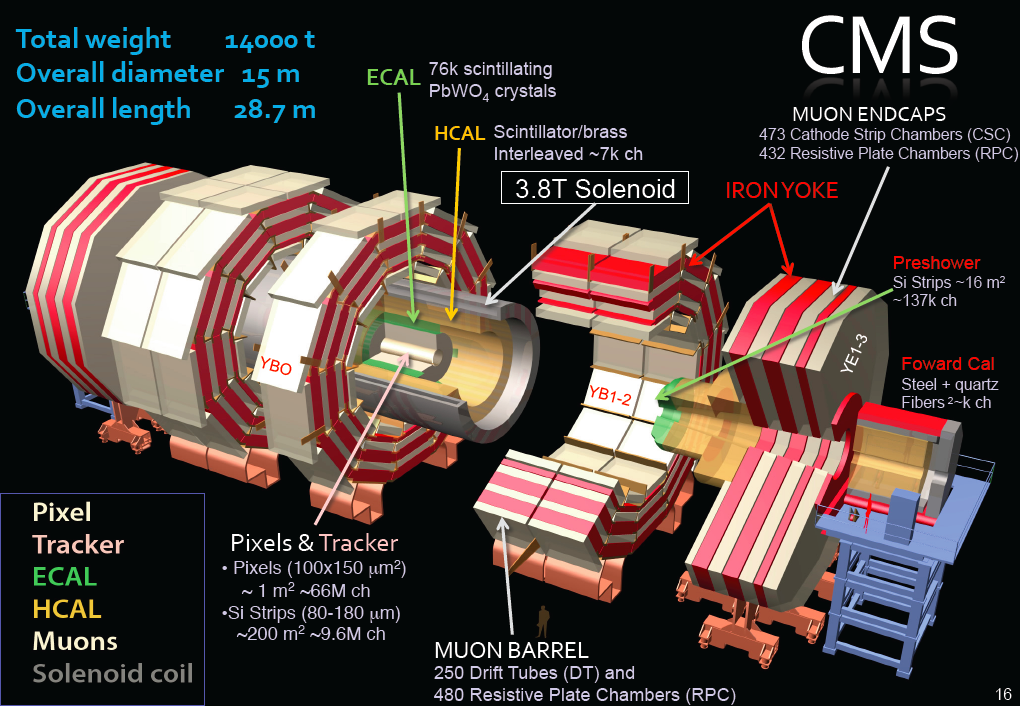
\includegraphics[width=\linewidth]{images/CMSDiagram.png}
  \end{center}
\end{minipage}

\end{center}
}


\headerbox{The $\gamma\gamma$ channel}{name=ggChannel,span=2,column=0,below=CMSExperiment}{

\begin{minipage}{0.60\linewidth}
{\smaller
In the $H \rightarrow \gamma\gamma$ analysis a search is made for a narrow peak in the diphoton invariant mass
distribution in the range 110–150 GeV, sitting on a large background:
  {\smaller[2]
  \begin{itemize}
   \item Large irreducible background from QCD production of two photons;
   \item Reducible background where one or more of the reconstructed photons originate from misidentification of jet fragments
  \end{itemize}
  }
Early detailed studies indicated this to be one of the most promising channels in the search for a SM Higgs boson in the 
low-mass range.

}

\vspace{5px}

{\tiny
\textbf{Figure 2:}  Event recorded with the CMS detector in 2012 at a proton-proton centre-of-mass energy of 8 TeV. The event shows characteristics expected from
the decay of the SM Higgs boson to a pair of photons. 

}


\end{minipage}
\hspace{1px}
\begin{minipage}{0.37\linewidth}
  \begin{center}
    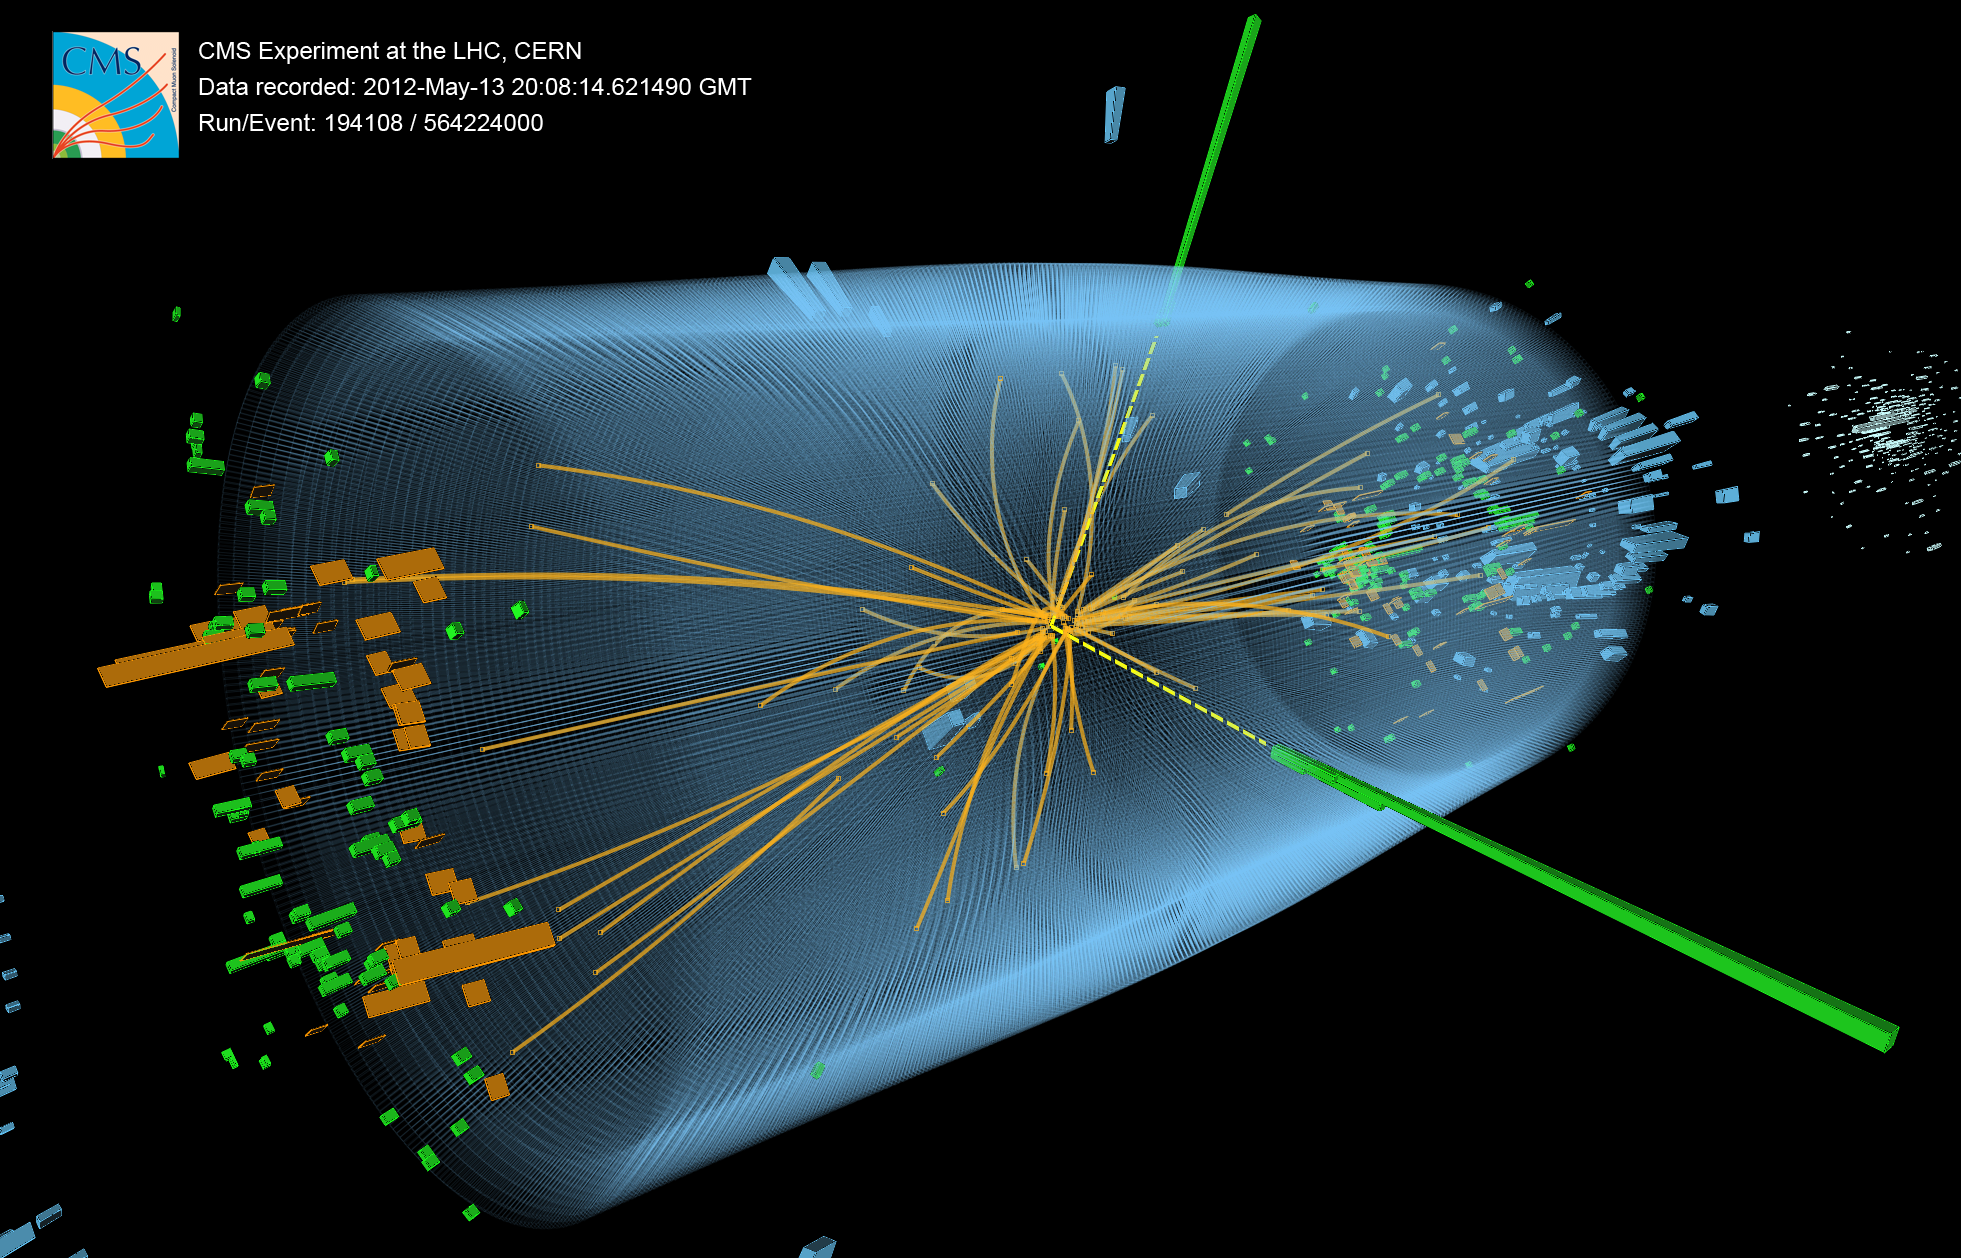
\includegraphics[width=\linewidth]{gammagamma_run194108.png}
  \end{center}  
\end{minipage}

}


\headerbox{The challenge}{name=SSB,column=0,row=0,above=ggChannel}{
The current knowledge on the field of particle physics is summarized in the Standard Model (SM). 
This model is incomplete without the inclusion of a spontaneous symmetry breaking mechanism that would explain the 
observation that the electroweak bosons (the W and Z particles) have mass. This can be done with the Higgs Mechanism, 
which suggests the presence of new previously unobserved particle, the Higgs Boson.
}

\headerbox{Event categorization}{name=EventCategorization,span=1,column=2,below=CMSExperiment}{
  {\smaller
Candidate diphoton events are separated into mutually exclusive categories of different expected 
signal-to-background ratios, based on the properties of the reconstructed photons and on the 
presence of two jets satisfying criteria aimed at selecting events in which a Higgs boson is produced 
through the VBF process. The analysis uses multivariate techniques for the selection and classification of 
the events. As an independent cross-check, an analysis is also performed, using simpler criteria based on the 
properties of the reconstructed photons to select and classify events. The multivariate analysis achieves 
15\% higher sensitivity than the cross-check analysis.

}
}

\headerbox{Expected yields}{name=MVATable,span=1,column=2,below=EventCategorization}{
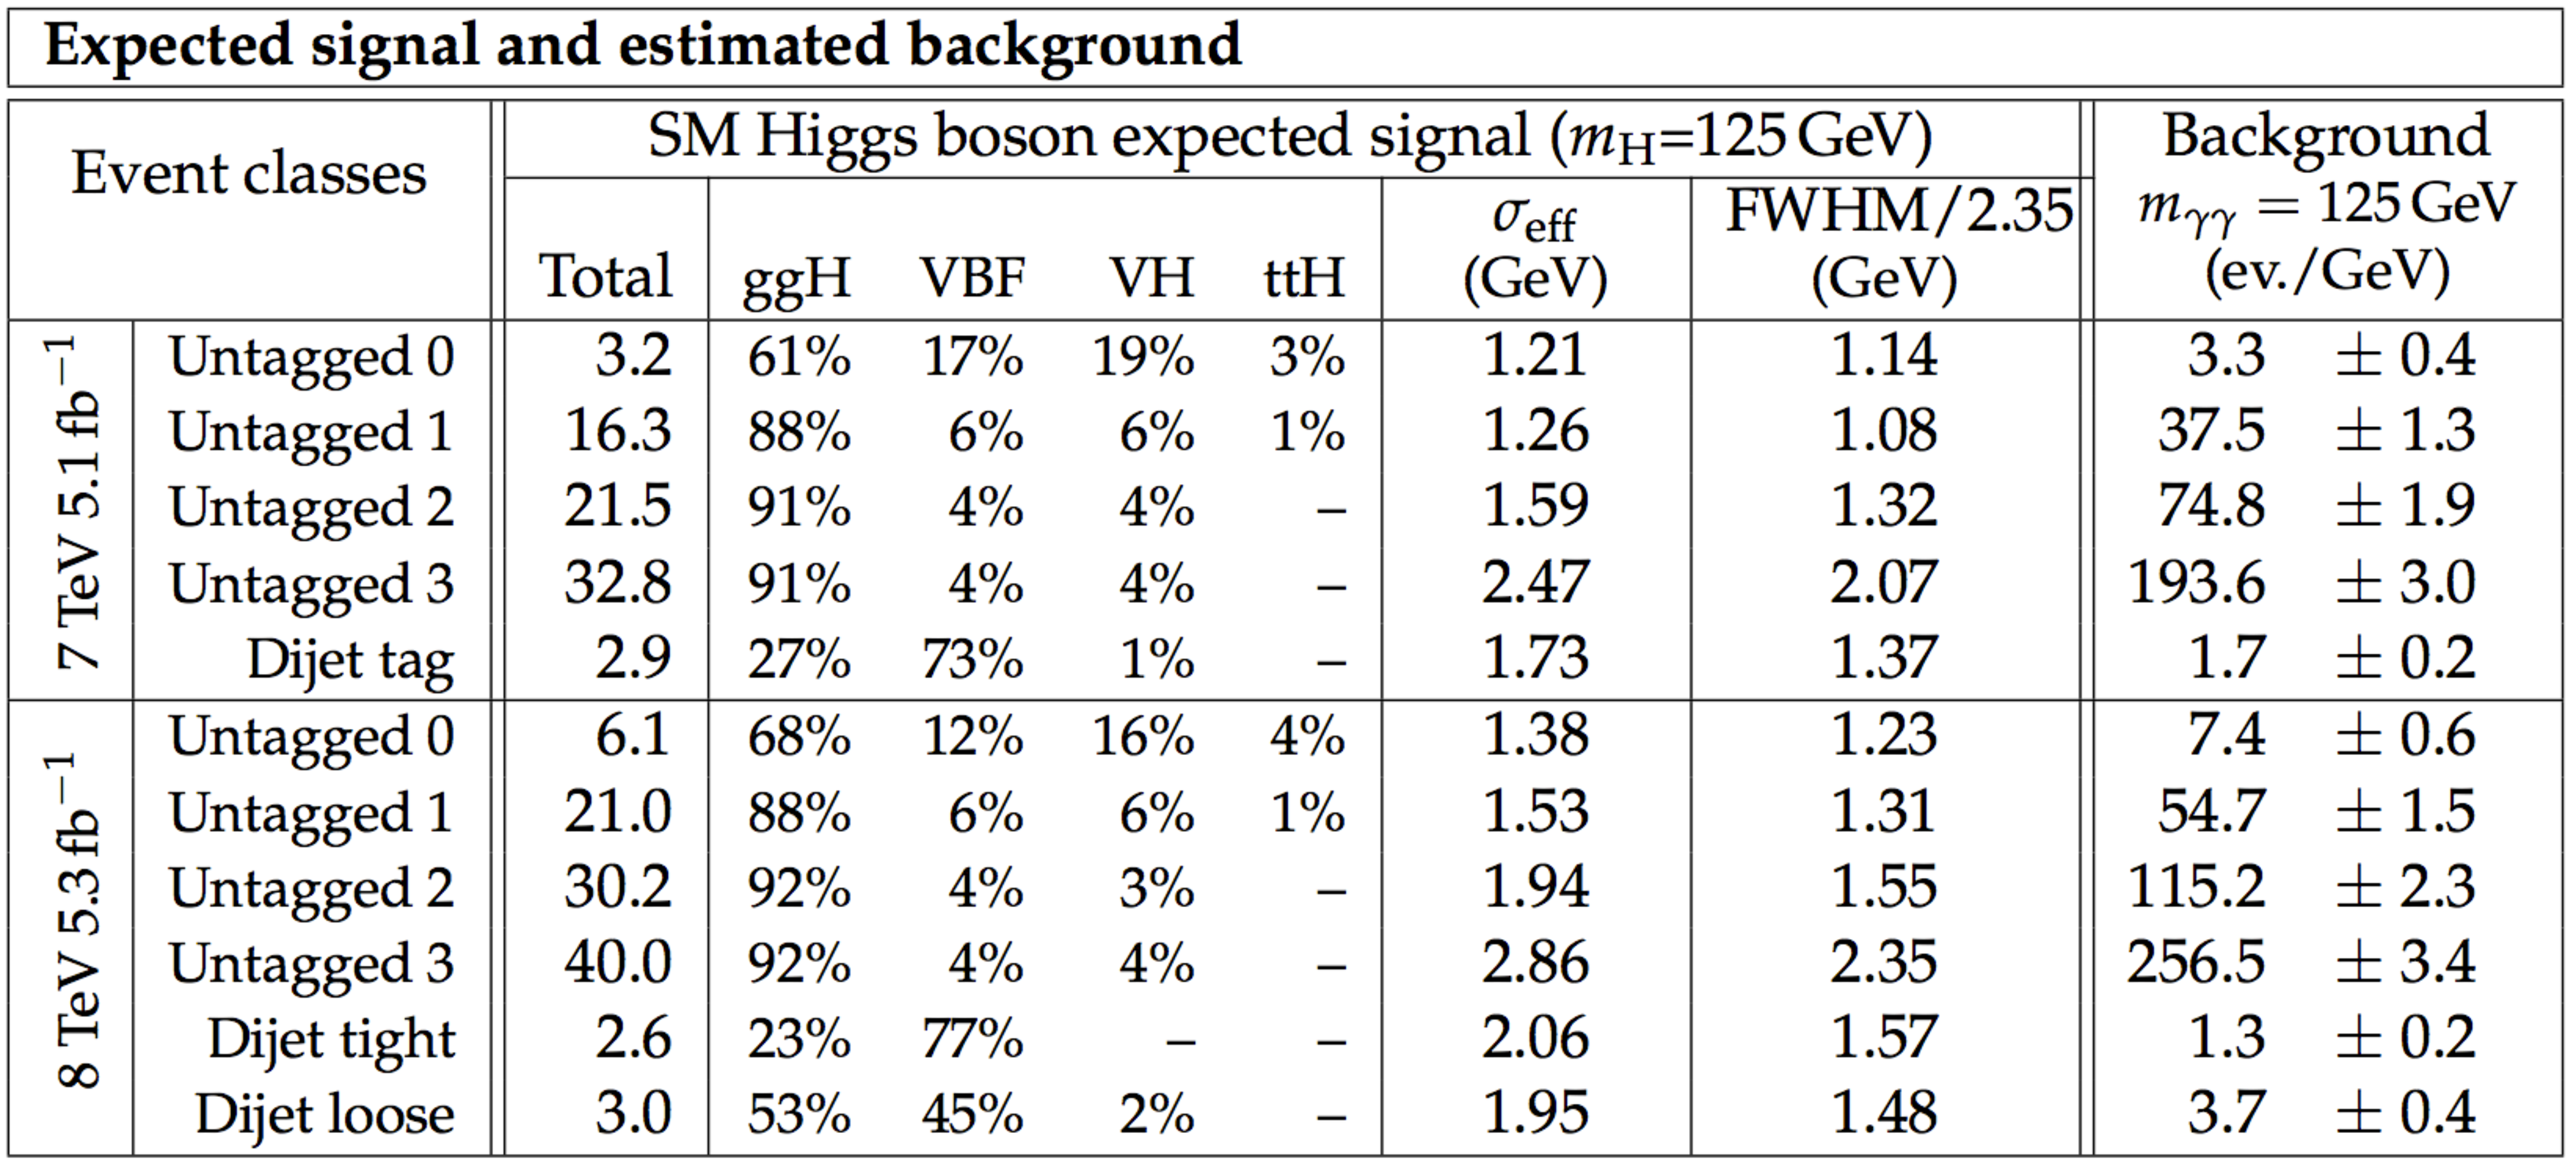
\includegraphics[width=\linewidth]{tables/table_SMHiggs_ExpectedEventsAndResolution.pdf}
{\tiny
\textbf{Table 1:} Expected numbers of SM Higgs boson events $(m_H=125$ $GeV$) and estimated back-
ground (at $m_{\gamma\gamma}=125$ $GeV$) for all event categories of the 7 and 8 $TeV$ data sets.

}
}

\headerbox{Invariant mass}{name=InvMass,span=1,column=2,below=MVATable}{
\centering
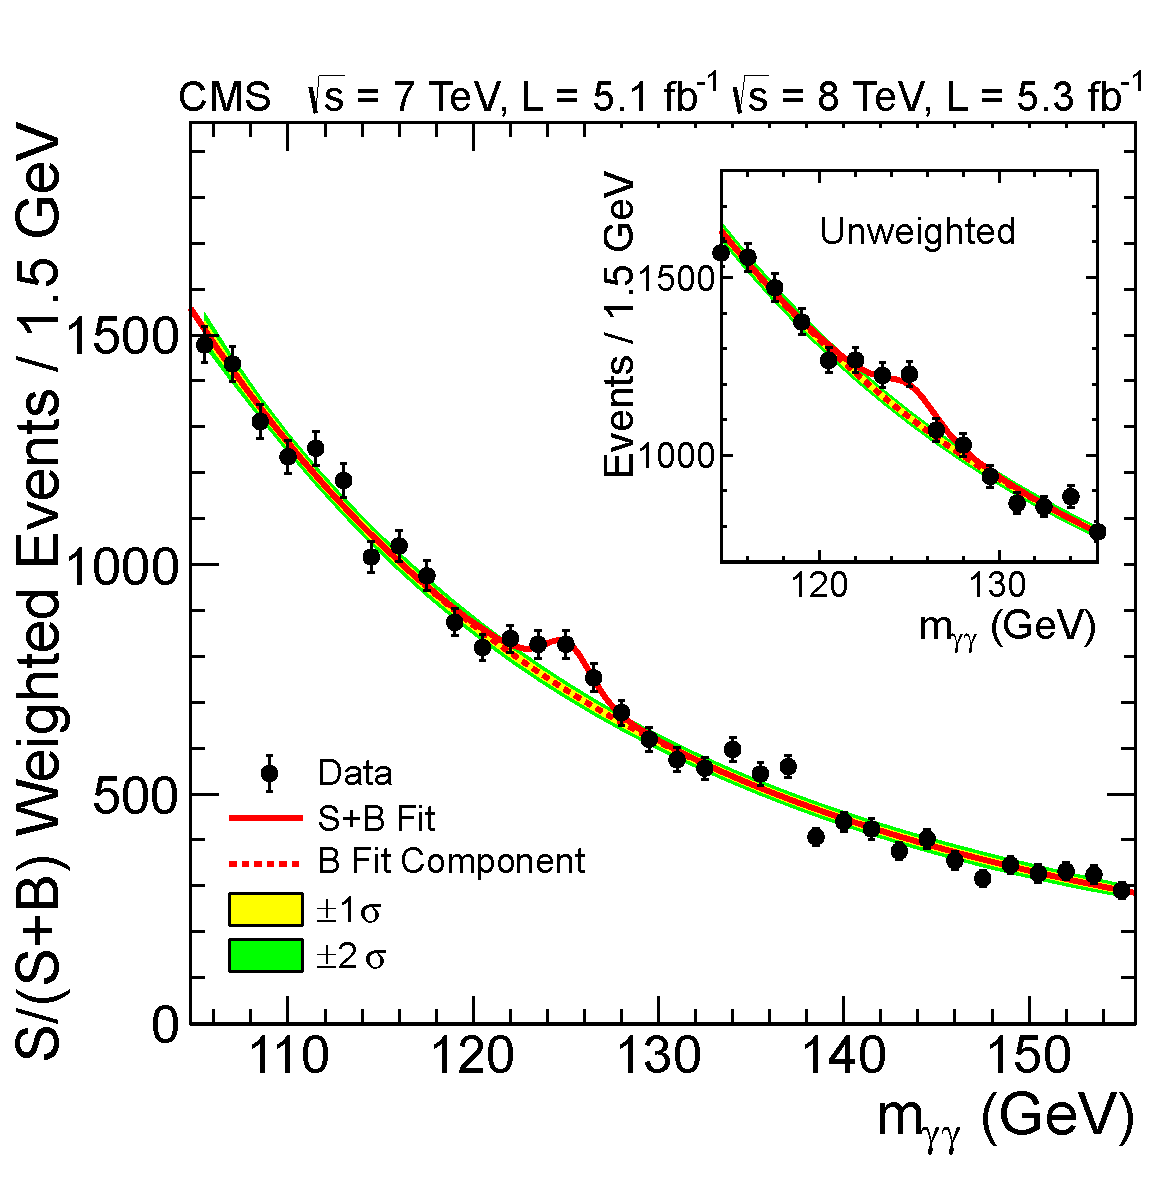
\includegraphics[width=0.80\linewidth]{images/figure_WeightedDiphotonInvMass.pdf} \\
{\tiny
\textbf{Figure 3:} The diphoton invariant mass distribution with each event weighted by the $S/(S + B)$ value of 
its category. The lines represent the fitted background and signal, and the coloured bands represent the $\pm1$ and $\pm2$ 
standard deviation uncertainties on the background estimate. The inset shows the central part of the unweighted invariant 
mass distribution.
  
 }
}

\headerbox{References}{name=references,column=2,below=InvMass}{
\smaller[2]						% Make the whole text smaller
\vspace{-0.4em} 					% Save some space at the beginning
\bibliographystyle{plain}				% Use plain style
\renewcommand{\section}[2]{\vskip 0.05em}		% Omit "References" title
\begin{thebibliography}{1}				% Simple bibliography with widest label of 1
\setlength{\baselineskip}{0.4em}			% Save space with longer lines
\itemsep=-0.01em					% Save space between the separation
\bibitem{old_Hgg} The CMS Collaboration: \emph{Search for the standard model Higgs boson decaying into two photons in pp collisions at sqrt(s)=7 $TeV$}, CMS-HIG-11-033, CERN-PH-EP-2012-024, arXiv:1202.1487v1 [hep-ex]
\bibitem{article_NewBoson} The CMS Collaboration: \emph{Observation of a new boson at a mass of 125 $GeV$ with the CMS experiment at the LHC}, CMS-HIG-12-028, CERN-PH-EP-2012-220, arXiv:1207.7235v1 [hep-ex]

\end{thebibliography}
}

\headerbox{Acknowledgements}{name=acknowledgements,column=2,below=references, above=bottom}{
{\smaller[2]			
The author thanks the Portuguese Government through Fundação para a Ciência e a 
Tecnologia (SFRH/BD/77979/2011) for supporting this research.

}
} 



\headerbox{Event selection}{name=EventSelection,span=2,column=0,below=ggChannel}{
{\smaller
The event selection requires two photon candidates satisfying:
  {\smaller[2]
  \begin{itemize}
    \item A $p_T$ threshold for photon leading (subleading) of $m_{\gamma\gamma}/3$ ($m_{\gamma\gamma}/4$). Events 
          passing the dijet selection, the requirement on the leading photon is $m_{\gamma\gamma}/2$;
    \item ``Loose'' photon identification criteria;
    \item Photons reconstructed within the fiducial region $|\eta|<2.5$ (excluding barrel-endcap transition $1.44<|\eta|<1.57$);
  \end{itemize}
  }
Jet selection criteria are applied to the two jets of largest $p_T$ in the event within $|\eta|<4.7$:
  {\smaller[2]
  \begin{itemize}
    \item $p_T$ thresholds for the two jets are 30 and 20 $GeV$;
    \item $\eta$ separation is required to be greater than 3.5;
    \item The dijet invariant mass is required to be greater than 350 and 250 $GeV$
          for the 7 and 8 $TeV$ data sets;
  \end{itemize}
  }
  
  Additional pseudorapidity and agular requirements are made to the selected jets, dijet and diphoton.
  
%   Two additional selection criteria, relating the dijet to the diphoton system, are applied: the difference 
% between the average pseudorapidity of the two 
% jets and the pseudorapidity of the diphoton system is required to be less than 2.5, and the difference
% in azimuthal angle between the diphoton system and the dijet system is required to be greater
% than 2.6 radians.

  Events containing a dijet are put at a single category t 7 $TeV$ and 2 categories at 8 $TeV$ where the 
  separations is based on the dijet invariant mass and jet $p_T$

% A multivariate regression is used to extract the photon energy and a photon-by-photon estimate
% of the uncertainty in that measurement.
}
}

\headerbox{Multivariate analysis}{name=MVA,span=2,column=0,below=EventSelection}{
{\smaller

For the multivariate analysis, a boosted decision tree (BDT) is trained to give a high
output value (score) for signal-like events and for events with good diphoton invariant mass
resolution, based on the following observables:

  {\smaller[2]
  \begin{itemize}
    \item The photon quality determined from electromagnetic shower shape and isolation variables;
    \item The expected mass resolution;
    \item The per-event estimate of the probability of locating the diphoton vertex within 10 $mm$ of its true
location along the beam direction;
    \item kinematic characteristics of the photons and the diphoton system;
  \end{itemize}
  }

The kinematic variables are constructed so as to contain no information about the invariant mass of the 
diphoton system. The diphoton events not satisfying the dijet selection are classified into five categories 
based on the output of the BDT, with category boundaries optimized for sensitivity to a SM Higgs boson. 
Events in the category with smallest expected signal-to-background ratio are rejected, leaving four categories 
of events.

}
}

\headerbox{Results}{name=Results,span=1,column=0,below=MVA,above=bottom}{
\smaller  
The diphoton invariant mass distribution shown in Fig. 3 clearly shows an excess at mass of 125 $GeV$. A fit is 
preformed to the diphoton mass distribution in each category, with the background modeled using a polynomial and the 
signal using a parametric model from Monte Carlo simulation.

The local p-value is shown as a function of $m_H$ in Fig. 4 for the 7 and 8 $TeV$ data, 
and for their combination. The expected significance of the local p-value for a SM Higgs boson of mass
125 $GeV$ is 2.8 $\sigma$. The minimum local p-value corresponding to the upward fluctuation of the observed limit
at 125 $GeV$ corresponds to $4.1 \sigma$. The significances of the corresponding minimum local p-values seen with 
the sideband-background-model and the cross-check analysis are 4.6 $\sigma$ at $m_H=125$ $GeV$ and 3.7 $\sigma$ 
at $m_H=124$ $GeV$, respectively. The best-fit signal strength for a SM Higgs boson mass hypothesis of 125 
$GeV$ is $\sigma/\sigma_{SM}=1.6 \pm 0.4$.

The excess is most significantly seen also in the ZZ decay channel, which together with $\gamma\gamma$ are the 
channels with best mass 
resolution. A fit to these signals gives a mass of $125.3 \pm 0.4 (stat.) \pm 0.5 (syst.)$ $GeV$. The decay to 
two photons indicates that the new particle is a boson with spin different from one.

}

\headerbox{p-Value}{name=pValue2,span=1,column=1,below=MVA,above=bottom}{
\begin{center}
  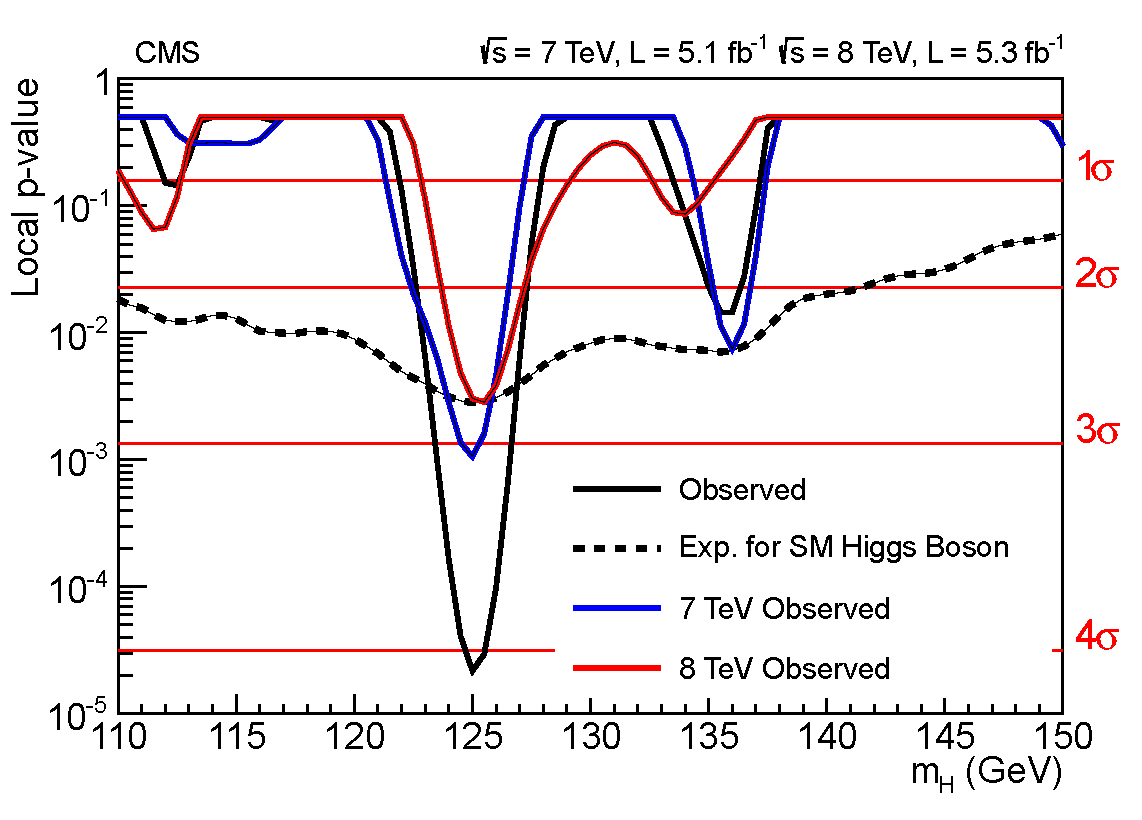
\includegraphics[width=\linewidth]{images/figure_LocalValues.pdf}   
\end{center}
  {\tiny
  \textbf{Figure 4:} The local p-value as a function of $m_H$ in the $\gamma\gamma$ decay mode for the combined 7 and
8 $TeV$ data sets. The dashed line shows the expected local p-value for the combined data sets, should a SM
Higgs boson exist with mass $m_H$.

}

}

\end{poster}
\end{document}
